
\begin{enumerate}[label=\thesection.\arabic*.,ref=\thesection.\theenumi]
\numberwithin{equation}{enumi}
\numberwithin{figure}{enumi}
\numberwithin{table}{enumi}
\item During the lockdown period,many families got bored of watching TV all the time.Out of these families, one family of 6 members decided to play a card game.17 cards numbered 1,2,3,4,..,17 are put in a box and mixed thoroughly.One card is drawn by one member at random and other family members bet for the chances of drawing the number either prime,odd or even etc.
\begin{figure}[H]
\centering
	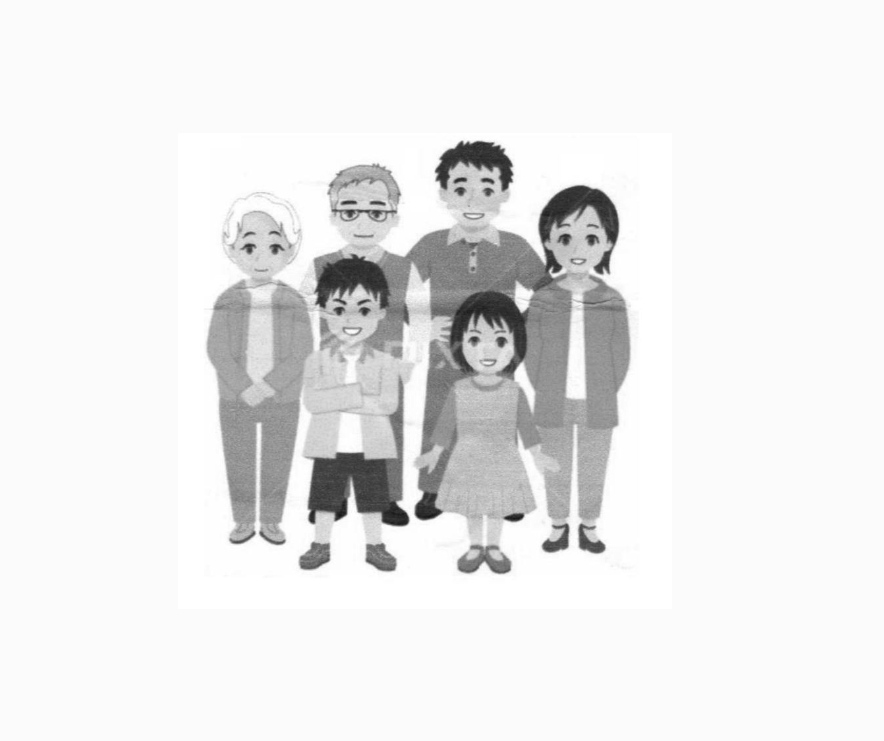
\includegraphics[width=\columnwidth]{figs/satish.jpg}                                                                                              
\caption{Family of six}
\label{fig:satish.jpg}                                                                                                                      \end{figure}
Based on the above,answer the following questions:
\begin{enumerate}[label=(\roman*)]                                                                                                                                         \item The first member of the family draws a card at random and another member bets that it is an even prime number.What is the probability of his winning the bet?                                                                                                                           \begin{enumerate}[label=(\Alph*)]
        \item $\frac{2}{17}$
        \item $\frac{3}{17}$
        \item $\frac{1}{17}$
        \item $\frac{4}{17}$
\end{enumerate}
       \item The second member of the family draws a card at random and some other
member bets that it is an even number. What is the probability of his winning
the bet ?
\begin{enumerate}[label=(\Alph*)]
        \item $\frac{7}{17}$
        \item $\frac{8}{17}$
        \item $\frac{9}{17}$
        \item $\frac{10}{17}$
\end{enumerate}
      \item What is the probability that the number on the card drawn at random is
divisible by 5 ?
\begin{enumerate}[label=(\Alph*)]
        \item $\frac{5}{17}$
        \item $\frac{4}{17}$
        \item $\frac{3}{17}$
        \item $\frac{2}{17}$
\end{enumerate}
      \item What is the probability that the number on the card drawn at random is a
multiple of 3 ?
\begin{enumerate}[label=(\Alph*)]
        \item $\frac{5}{17}$
        \item $\frac{6}{17}$
        \item $\frac{7}{17}$
        \item $\frac{8}{17}$
\end{enumerate}                                                                                                                                         \end{enumerate}
\item \begin{enumerate}[label=(\alph*)]
\item Two different coins are tossed simultaneously. Write all the possible outcomes.                                                                   
\item A die is thrown once. Write the probability of getting a number less than $7$.
\end{enumerate}
\item  If the probability of occurrence of event E,\pr{E}=0.99, what is the probability of non-occurrence of the event E,\pr {not E}?                   \item \begin{enumerate}[label=(\alph*)]
\item A bag contains 5 white balls and 7 red balls.A ball is drawn at random from the bag.What is the probability that it is either a white or a red ball?
\item Two coins are tossed together once.What is the probability of getting at least one head?
\end{enumerate}
\item Cards marked with numbers $1$,$2$,$3$,$4$, ..., $100$ are placed in a bag and mixed together throughly. A card is randomly drawn from the bag.Find the probability that the numbers on the card is                             \begin{enumerate}[label=(\roman*)]                                                                                                                     \item an even number,
\item a $2$-digit number,
\item a perfect square.                                         
\end{enumerate}
\item \begin{enumerate}[label=(\alph*)] 
\item How many outcomes are possible when three dice are thrown together?
\item if \pr{E}=0.015, then find \pr{not E}.
\end{enumerate}
\item  During summer break, Harish wanted to play with his friends but it was too hot outside, so he decided to play some indoor game with his friends. He collects $20$ identical Icards and writes the numbers $1$ to $20$ on them (one number on one card). He puts them in a box. He and his friends make a bet for the chances of drawing various cards out of the box. Ench was given a chance to tell the probability of picking one card out of the box.

Based on the above,answer the following questions:
\begin{enumerate}[label=(\roman*)]                                                                                                                                  \item The probability that the number on the card drawn is an odd prime number,is
\begin{enumerate}[label=(\Alph*)]                            

          \item $\frac{3}{5}$
          \item $\frac{2}{5}$
          \item $\frac{9}{20}$                      
          \item $\frac{7}{20}$                                               \end{enumerate}
\item The probability that the number on the card drawn is a composite number is
\begin{enumerate}[label=(\Alph*)]
        \item $\frac{11}{20}$                     
	\item $\frac{3}{5}$                       
	\item $\frac{4}{5}$                     
	\item $\frac{1}{2}$
\end{enumerate}
\item The probability that the number on the card drawn is a multiple of $3$,$6$ and $9$ is
\begin{enumerate}[label=(\Alph*)]                 
	\item $\frac{1}{20}$                      
	\item $\frac{1}{20}$                      
	\item $\frac{3}{20}$                      
	\item $0$
\end{enumerate}
\item The probability that the number on the card drawn is a multiple of $3$ and $7$is
\begin{enumerate}[label=(\Alph*)]                 
	\item $\frac{3}{10}$                      
	\item $\frac{1}{10}$                      
	\item $0$
        \item $\frac{2}{5}$               
\end{enumerate}                                                              \item If all cards having odd numbers written on them are removed from the box and then one card is drawn from the remaining cards, the probability of getting a card having a prime number is
\begin{enumerate}[label=(\Alph*)]                 
	\item $\frac{1}{20}$
	\item $\frac{1}{10}$                      
        \item $0$ 
        \item $\frac{1}{5}$               
\end{enumerate}
\end{enumerate}
\item \begin{enumerate}[label=(\alph*)]
\item In a single throw of a pair of dice,find the probability that both dice have the same number.
\item A card is drawn from a well-shuffled pack of $52$ cards.Find the probability that it is not an ace.
\end{enumerate}
\end{enumerate}
